% boosting.tex
% Jeremy Barnes, 29/8/1999
% $Id$

% The chapter of my thesis on Boosting

\chapter{Boosting and similar algorithms}
\label{chapter:boosting}

The name ``Boosting'' is applied to many different machine learning
algorithms, which combine many weak hypotheses to form a ``strong''
hypothesis that significantly outperforms them.

We first describe the classic algorithm \emph{AdaBoost}.  A full
description is given, along with some examples of its performance and
a discussion of why it performs so well.  We also give a formal
definition of what we mean by the term ``boosting''.

A useful viewpoint of the boosting algorithm as an optimisation via
gradient descent in a cost space is then considered.  A result from
Mason et al. \cite{Mason99} is derived which shows that boosting is
indeed performing gradient descent.

We then consider \emph{normed boosting algorithms} where the
weights of the hypotheses are constrained by some norm.  Several
properties of these algorithms which are different from those of
unconstrained boosting algorithms are discussed.

We then turn to questions of the performance of boosted algorithms; in
particular guarantees on the training and generalisation error.
Several results are presented.

Finally, we motivate the $p$-boosting algorithm by considering the
problem of overfitting in boosting.  Both practical and theoretical
explanations for this phenomenon are given.


\section{The AdaBoost algorithm}

We first describe the AdaBoost algorithm, first published by Freund
and Scahpire \cite{Freund96}.  In essence, this algorithm
``bootstraps'' itself onto another learning algorithm (the \emph{weak
learning algorithm}) and improves the performance by producing a
linear combination of weak learning hypotheses.

AdaBoost performs \emph{very} well; its combined hypotheses generally
perform significantly better than \emph{any} non-boosted algorithm.
This is particularly true for reliable (low-noise) data.  Even
the simplest of weak algorithms, when ``boosted'', will usually
outperform the best unboosted algorithms.
\footnote{As a result, the focus of recent research effort has shifted
from the development of \emph{learning} algorithms (which are all more 
or less equivalent when boosted) to the development of better
\emph{boosting} algorithms.}

We consider questions of how and why AdaBoost works; in
particular how it chooses the optimal linear combination of
classifiers from the very large set of possible linear combinations.

Figure \ref{fig:boosting algorithm} gives an explicit description of
AdaBoost.  The key features are:
%
\begin{enumerate}
\item	The AdaBoost algorithm operates in iterations.  During
	iteration $t+1$, one classifier $h_{t+1}$ is added to the combined
	hypothesis $F_{t}$, to give $F_{t+1} = F_t + b_t h_{t+1}.$
\item	The weight $b_t$ of each weak hypothesis (the \emph{classifier
	weight}) depends upon the weighted empirirical risk
	(\ref{eqn:weighted empirical risk}) of that classifier on the
	training dataset.  Section \ref{sec:classifier weights}
	describes these classifier weights in more detail. 
\item	Each sample in the training dataset is given a weight
	(\emph{sample weight}) which is modified depending upon how
	``hard'' that sample is to classify.  Section \ref{sec:sample
	weights} describes these sample weights in more detail.
\end{enumerate}
%
First, we explain our notation.


\begin{linefigure}
\label{fig:boosting algorithm}
\noindent{\bf Input:} $m$ examples $X = ((\bfx_1, y_1), \ldots, (\bfx_l,
y_m))$ and a weak learning algorithm $\bbW$
\par
\noindent{\bf Initialisation:} $F_0(\bfx) = 0$; $w_i|_0 = 1/m$ for
$i=1 \ldots m$ 
\par
\noindent {\bf Do for} $t=1 \ldots T$:
\par
\noindent Update $F_t \trainboost F_{t+1}$: 
\par
\begin{enumerate}

\item	Train weak learner $\bbW$ on the weighted sample set 
	$(\bfx_1, y_1, w_1|_t) \ldots (\bfx_m, y_m, w_m)$
	and obtain weak learner $h_t(\cdot) : \calI \mapsto \{\pm 1\}$

\item	Calculate the weighted empirical risk (training error
	$\epsilon_t$) of $f_t(\cdot)$: 
	%
	\begin{equation}
	\epsilon_t = R_{\emp}^{w|_t}(h) = \sum_{j : h(\bfx_j) \neq
	y_j} w_j|_t
	\end{equation}

	If $\epsilon_t = 0$ (a single weak learner can correctly learn
	the relationship) or $\epsilon_t \geq 1/2$; thus the weak
	learner is performing as badly as random guessing) then abort
	the training process, with $\bbB_{t+1} = \bbB_{t}$.

\item	Calculate our classifier weight $b_t$:
	\begin{equation}
	b_t = - \frac{1}{2} \log \frac{\epsilon_t}{1 - \epsilon_t}
	\end{equation}

\item	Update the sample weights $w_i$:
	%
	\begin{equation}
	w_i|_{t+1} = \left\{
	\begin{array}{cl}
		\frac{w_i|_t}{Z_t} \exp \left\{ b_t \right\}&	\qquad \qquad \mbox{if 
		$f_t(x_i) = y_i$} \\
		\frac{w_i|_t}{Z_t} \exp \left\{ -b_t \right\} & \qquad \qquad
		\mbox{otherwise} \\
	\end{array} \right.
	\label{eqn:sample weight update}
	\end{equation}

	where $Z_t$ is a normalisation constant, such that
	$\sum_{i=1}^{l} w_i|_{t+1} = 1$
\end{enumerate}

\par
\noindent {\bf Output:} 
\begin{equation}
H(\bfx) = \sign (F(\bfx)) = \sign \left\{ \sum_{i=1}^T b_i f_i(\bfx) \right\}
\end{equation}
\caption{The AdaBoost algorithm $\bbB$}
\end{linefigure}


\subsection{Notation}

The notational conventions mentioned here refer to the algorithm
printed in figure \ref{fig:boosting algorithm}.

\begin{itemize}
\item	The AdaBoost algorithm is given the symbol $\bbB$, and the
	weaklearner $\bbW$.
\item	The sample weights are denoted $w_i|_t$, where $i \in 1 \ldots
	m$ is the sample number and $t$ the iteration number.
\item	The classifier weights are denoted $b_1 \ldots b_t$.
\item	The non-thresholded hypothesis is $F(\cdot)$; the output of
	the algorithm is $H(\cdot) = \sign(F(\cdot))$ (similar
	notation to the individual hypotheses).
\item	The process of training AdaBoost for one iteration is denoted
	$F_t \trainboost F_{t+1}$.
\end{itemize}

Two AdaBoost hypotheses are said to be \emph{equivalent} ($\equiv$) if
they produce the same output for all input, even if their internal
state ($b$ and $w$ values) are not identical.


\subsection{Classifier weights}
\label{sec:classifier weights}

The AdaBoost algorithm combines a number of ``weak'' classifiers
$h_1(\cdot), \ldots, h_n(\cdot)$ in a linear combination to produce a
``stronger'' classifier $F(\cdot) = \sum_{i=1}^{n} b_i h_i(\cdot)$.
The coefficients $b_i$ are subject to the condition that they produce a
convex combination where $\|b\|_1 = \sum_{i=1}^{t} b_i = 1$.

AdaBoost's training process is divided into iterations.  On iteration
$t$, one weak learner $h_t(\cdot)$ is added to the linear
combination ($h_t$ is chosen by the weak learning algorithm).  The
coefficient $b_t$ of $h_t$ is calculated from the 
training error $\epsilon_t$ of $h_t$ as 
%
\begin{equation}
b_t = - \log \frac{\epsilon_t}{1 - \epsilon_t}
\label{eqn:theory:bt}
\end{equation}
%
This function is plotted in figure \ref{fig:b function}.

\begin{linefigure}
\begin{center}
\includegraphics{figures/classifier_weights.epsg}
\end{center}
\begin{capt}{Classifier weights against weighted training error}
When $\epsilon_t = 1/2$, the classifier only does as well as random
guessing, and $b_t = 0$.  As $\epsilon_t$ approaches zero, $b_t$
increases without bound.  The effect is that $F$ becomes dominated by
those weak hypotheses that performed well on the training samples
(training is halted if $\epsilon_t = 0$ or $\epsilon_t \geq
1/2$).
\end{capt}
\end{linefigure}


\subsection{Sample weights}
\label{sec:sample weights}

Each sample in the training set has a corresponding weight $w_j$ which
is updated to reflect the difficulty of that sample.  On each iteration the
weights of samples which $h_t$ classified incorrectly are increased
(scaled by $\exp \{ -b_t \}$); the whole lot are then normalised.
This function has the following effect on distribution of weights:

\begin{itemize}

\item	Training samples which are misclassified often, or are one of 
	few points to get misclassified, increase their proportion of
	the weight (are identified as ``hard samples'');

\item	Other samples decrease their proportion of the weight, and are
	identified as ``easy'' samples.

\end{itemize}

\begin{linefigure}
\begin{center}
\includegraphics{figures/sample_weights.epsg}
\end{center}
\begin{capt}{Evolution of sample weights}
The figure shows the evolution of the sample weights from (a) 10
iterations to (b) 100 iterations of boosting over a set of training
data in $\bbR^2$.  The sample weight at a point is proportional to the
intensity of the dot.  The weights of those samples far from the
decision boundary (indicated) approach zero as $t \rightarrow \infty$.
\end{capt}
\end{linefigure}

The overall effect is for those samples near the decision boundary to
increase in weight, and those far from it to decrease.  This forces
the algorithm to concentrate on the hard samples, and is one reason
why it works well on low-noise datasets.  Unfortunately, those samples
corrupted by noise are usually hard also, and concentrating on those
is not desirable. (clarify)

\subsection{Summary}


\section{Boosting as gradient descent}
\label{sec:theory:gradient descent}

Recent work has shown boosting to be an implementation of a gradient
descent algorithm in an inner product space
\cite{Mason99}\footnote{This discussion follows Mason et
al. \cite{Mason99} rather closely with some changes in notation and
omission of details such as stopping criteria.}.  An inner product
space requires both a universal set $\mathcal{X}$ and an inner product
operator \ip{\cdot}{\cdot}.  We define
%
\begin{equation}
\calX = 
\mathrm{co} (\calF) \doteq
 \bigcup _{n \in \mathbb{N}}
\left\{
 \sum_{i=1}^{n}
  b_i
f_i : f_1, \ldots, f_n \in \calF,
 b_1, \ldots, b_n \in \mathbb{R},
 \sum_{i=1}^{n} | b_i | = 1
\right\} \cup \emptyset
\end{equation}
%
(which is the convex hull of \calF), and
%
\begin{equation}
\ip{F}{G} = \frac{1}{l} \sum_{i=1}^{l} F(\bfx_i)G(\bfx_i) \qquad
F, G \in \calX
\label{eqn:inner product definition}
\end{equation}
%
We also choose the cost function
%
\begin{equation}
C(F) = \frac{1}{l} \sum_{i=1}^{l} \exp
\left\{ -y_i F(\bfx_i) \right\}
\label{eqn:theory:cost function}
\end{equation}

At iteration $t$ of gradient descent, we wish to choose a hypothesis $h_t$ and
a weight $b_t$ such that $C(F + b_t h_t)$ decreases (the choice of
$h_t$ is made indirectly through the choice of the sample weights
$w|_t$).  In other words, we are asking for sample weights $w|_t$ that
choose a \emph{direction} $h_t \in \calH$ such that $C(F + b_t h_t)$
decreases as fast as possible.  This direction is the negative of the
functional derivative of $C$:
%
\begin{equation}
f = -\nabla C(F)(\bfx) = \left. \frac{\partial C(F + \alpha
1_{\bfx})}{\partial \alpha} \right|_{\alpha = 0}
\label{eqn:functional derivative}
\end{equation}
%
where $1_{\bfx}$ is the indicator function of $\bfx$; this is
necessary as we can only evaluate \ref{eqn:functional derivative} at
points where we have a sample.  Since the optimal $h_t$ will not
necessarily be in $\calH$, we choose the $h \in \calH$ with the
greatest inner product $\ip{-\nabla C(F)}{h}$.  Under the inner
product space and cost functions we have chosen, we are maximising
%
\begin{equation}
- \ip{\nabla C(F)}{f} = - \frac{1}{m^2} \sum_{i=1}^{m} y_i f(\bfx_i)
  C'(y_i F(\bfx_i))
\label{eqn:function to maximise}
\end{equation}
%
The following theorem states that the \emph{weighted empirical risk}
$R_{\emp}^{w}$ (section \ref{sec:weighted empirical risk}) is the
``right'' form of risk to minimise, and gives the weights $w$.

\begin{theorem}[Weighted empirical risk minimisation]
Maximising (\ref{eqn:function to maximise}) is equivalent to
minimising the weighted empirical risk
%
\begin{equation}
R_{\emp}^{w_{|t}} = \sum_{i:y_i \neq h(\bfx_i)}^{m} w_{i|t}
\end{equation}
%
where $w_{|t}$ are
%
\begin{equation}
minus the derivative of the cost function
\label{eqn:gradient sample weights}
\end{equation}

\proof See \cite{Mason99}.  We assume that our cost function is
monotonically decreasing; the result follows easily from that
assumption.
\end{theorem}

Note that these weights are the same that AdaBoost uses.

Having chosen our direction, we now choose a step size $b_t$.
AdaBoost uses a line search for the minimum of the cost functional
along the line
%
\begin{equation}
b_t = \arg \min_{b_t} \sum_{i=1}^{m} C(y_i F(\bfx_i) + y_i b_t h_t(\bfx_i)
\end{equation}
%

which (for the cost function (\ref{eqn:theory:cost
function})) has a closed-form solution  (\ref{eqn:theory:bt}).  Thus, the
boosting algorithm implements gradient descent.  The process is
illustrated in figure \ref{fig:gradient descent}.

\begin{linefigure}
\begin{center}
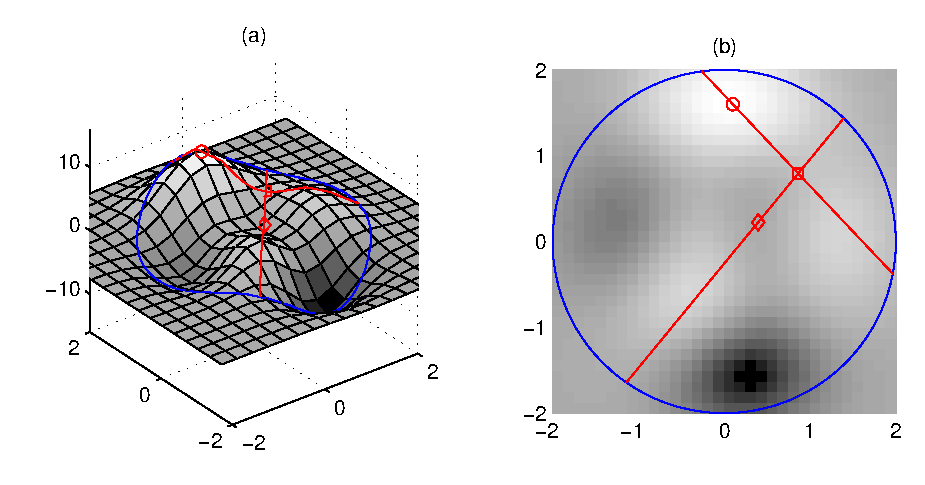
\includegraphics{figures/descent.epsg}
\end{center}
\begin{capt}{Schematic representation of gradient descent.}
Points within the circle are in \calH, the height of the surface
the value of (\ref{eqn:theory:cost function}) at that point.  (a) is a
3D view, (b) is top view. Lines show line searches; markers
minimums.  We descend from $\circ$ through $\Box$ to $\Diamond$, where
the algorithm terminates due to a local minima.
\end{capt}
\label{fig:gradient descent}
\end{linefigure}

This statement is formalised in the following theorem.

\begin{theorem}[AdaBoost implements gradient descent]
The AdaBoost algorithm implements gradient descent over a cost functional
%
\begin{equation}
Q(F, \bfx, y) = \exp \{-y F(\bfx) \}
\end{equation}
%
\proof We outline a skeleton, ignoring initial conditions and the
stopping conditions.  We will show that, given a state at iteration
$t$, then boosting and gradient descent produce identical states at
iteration $t+1$.

Once we have chosen $f_{t+1}$ using weighted empirical risk
minimisation, we need to choose $w_{t+1}$.  This is chosen to minimise
the cost functional along the line given by the direction $f_{t+1}$.
We can write the value of this cost functional as
%
\begin{equation}
C = \sum_{i=1}^{m} c \left( y_i F_t(\bfx_i) + y_i w_{t+1}
f_{t+1}(\bfx_i) \right)
\end{equation}
%
Substituting in $c(F(\cdot)) = e^{-yF(\cdot)}$, we obtain
%
\begin{equation}
C = \sum_{i=1}^{m} \exp \left\{ y_i F_t(\bfx_i) + y_i w_{t+1}
f_{t+1}(\bfx_i) \right\}
\end{equation}
%
Now we need to differentiate this expression with respect to
$w_{t+1}$.   This task is simplified considerably by noting that only
the second half of the exponential term is variable with $w_{t+1}$.
The result is that
%
\begin{eqnarray}{ll}
\label{eqn:differentiate}
\frac{\partial C}{\partial w_{t+1}} &
= & \sum_{i=1}^{m} \frac{\partial}{\partial w_{t+1}}
\exp \left\{ y_i F_t(\bfx_i) + y_i w_{t+1}
f_{t+1}(\bfx_i) \right\} \nonumber \\
& = & \sum_{i=1}^{m} y_i \exp \left\{ y_i F_t(\bfx_i) + y_i w_{t+1}
f_{t+1}(\bfx_i) \right\} 
\end{eqnarray}
%
From this result, we make several simplifications.  Noting that
%
\begin{equation}
y_i f_{t+1}(\bfx_i) = \left\{ 
	\begin{array}{ll}
	1 &	\qquad \mbox{if $y_i = f_{t+1}(\bfx_i)$} \\
	-1 &	\qquad \mbox{if $y_i \neq f_{t+1}(\bfx_i)$}
	\end{array}
\right.
\end{equation}
%
and that $w_{i | t} = k \exp \{ -y_i F_t(x_i) \}$ where $k$ is some
constant, we can recast (\ref{eqn:differentiate}) into the form
%
\begin{equation}
\underbrace{
	\frac{\sum_{i : y_i = f_{t+1}(\bfx_i)} w_{i|t}}
	     {\sum_{i : y_i \neq f_{t+1}(\bfx_i)} w_{i|t}}
}_{\epsilon_t}
= \exp \left\{ 2 \alpha \right\} 
\end{equation}
%
from which it is a simple transformation to obtain
(\ref{eqn:theory:bt}).  Thus, the state at iteration $t+1$ is
equivalent to boosting; thus boosting implements gradient descent.
\end{theorem}

The cost functional $c(\alpha) = e^{-\alpha}$ is an approximation to
the misclassification risk (\ref{eqn:misclassification risk}) that is
differentiable at all points and leads to a closed-form solution for
the step size.  It is plotted in figure \ref{fig:cost functional
approximation}.  Other approximations have been used; see Mason
et. al. \cite{Mason99} for details.

\begin{linefigure}
\begin{center}
\includegraphics{figures/cost_approx.epsg}
\end{center}
\begin{capt}{Approximation to the misclassification risk function}
The misclassification risk is plotted in the dotted line, with the
AdaBoost approximation plotted in the solid line.  It is clear that
the effect of this cost function will be to maximise the margins of
the samples.
\end{capt}
\label{fig:cost functional}
\end{linefigure}

\subsection{Summary}

In this section, we have shown that the AdaBoost algorithm implements
gradient descent.  There are four aspects of the gradient descent
problem that need to be specified:
%
\begin{enumerate}
\item	What is our universal set? (AdaBoost: $\co(\calH)$)
\item	What is our inner product? (AdaBoost: equation (\ref{eqn:inner
	product definition}))
\item	What is our cost function? (AdaBoost: $c(\alpha) =
	e^{-\alpha}$)
\item	How do we choose a step size? (AdaBoost: line search).
\end{enumerate}
%
In chapter \ref{chapter:development} we will consider changing some of
these to implement algorithms with desirable properties.

\section{AdaBoost and Boosting algorithms}

Until this point we have only considered the AdaBoost algorithm.  We
now extend our scope to other AdaBoost-like algorithms.  These
algorithms are termed ``boosting algorithms''.

There has recently been some debate over what constitutes a ``boosting
algorithm''; see for example Duffy and Helmbold \cite{Duffy99} who
adopt quite a restrictive definition.  In this thesis, we take a very
broad definition:

\begin{definition}[A boosting algorithm]
Any learning machine that constructs a hypothesis that is a linear
combination of base hypotheses by leveraging another learning machine
in an interative manner is a boosting algorithm.
\end{definition}

In particular, we don't require that the training error be guaranteed
to reach zero.  All algorithms considered in this thesis are,
according to definition \ref{def:boosting}, boosting algorithms.


\section{Properties of the AdaBoost and boosting algorithms}

We have covered the \emph{form} of the AdaBoost algorithm quite
extensively.  We now cover the \emph{function} of the algorithm, so
that we have a basis for comparison.

\subsection{Convergence properties}

This theorem provides two results.  The first, applicable to any
algorithm that implements gradient descent, shows that under certain
conditions on the cost function and step sizes the 
e main result of this section is a theorem that the empirical risk
(training error) of boosting will converge to zero if the algorithm is
trained for long enough.


This is from \cite{Schapire97}.  We use it to prove a theorem below.

\begin{theorem}[Weight update of AdaBoost]
The weights $w_{i|t}$ in the $t$-th iteration are chosen such that the
previous hypothesis has exactly a weighted training error $\epsilon$
of $1/2$.
\end{theorem}

The following theorem shows that the total weight of the boosting
algorithm is unbounded as the number of iterations increases.  It is
used to prove results on the minimum margin and final training error
of boosting.

\begin{theorem}
The size of the $b$ weight vector, $\|b\| \rightarrow \infty$
as $t \rightarrow \infty$ (assuming the boosting algorithm doesn't
terminate).

\proof ?
\end{theorem}

\begin{theorem}[Boosting reaches zero training error]
Given a weaklearner $\mathcal{L}$ and a training set $S$,
then either:
\begin{enumerate}
\item	The boosting algorithm will terminate; or
\item	There exists an iteration $t_{zero}$ such that for all $t \geq
	t_{zero}$ the training error $\epsilon_t = 0$.
\end{enumerate}

\proof If for any training iteration $t$ we have $\epsilon_t \geq 1/2$
then the boosting algorithm will terminate.  Assuming that this is not the
case, let us look at $\|b\|$.  As $t \rightarrow \infty$, $\|b\|
\rightarrow \infty$.  Thus, taking the normalised hypotheses $\bar{h}_i
= b_i \frac{h}{\sum b}$ we obtain
\[
C(F_{t+1}) = \sum_{i=1}^{m} \exp\left\{ -y_i b_i h_i(x_i)
\right\}^{\|b\|}
\]
Now, we know from theorem (number?) that the boosting algorithm will
always find the global minimum of the cost function.  Since all $b_i >
0$, this is achieved when all training examples are classified
correctly...

Need a lot more work on this proof.  Do I want to show that since it
gets steeper and steeper, the cost of a negative sample gets too
large?  I don't think that the way I am doing it is going to work,
really.  I need to show that because
\begin{itemize}
\item	The weights for wrong samples are increasing exponentially,
	and
\item	The power that the cost function is raised to makes the wrong
	margin get worse and worse,
\end{itemize}
then the thingy gets minimised...

I need to bring the training error < 1/2 into it somewhere.  I think
that I can show that if
\begin{itemize}
\item	$\|b\|$ increases without bound; and
\item	$\epsilon_t$ is always < 1/2, then we get there
\end{itemize}

I should look at Schapire's paper (I don't have it...); but I do want
to prove this in a way which uses the fact that the weight vector
grows to infinity (because I want to talk about that later).

\end{theorem}



\subsection{AdaBoost maximises the minimum margin}

This section introduces several theorems which together show that
AdaBoost chooses the linear combination that maximises the minimum
margin over its training samples.

\begin{theorem}[AdaBoost maximises the minimum margin]
Given a particular learning algorithm $F$ and a training
set $S$, define the minimum margin as
\[
m_{\min} = min_{\{x,y\} \in S} y_i F(x_i)
\]
Then the boosting algorithm will converge as $t \rightarrow \infty$ to
the solution which maximised the minimum margin.

\proof For boosting we can write $F_t = b_1 f_1 + \cdots + b_t f_t$.
Then defining our \emph{normalised hypotheses} $\bar{f}_i$ as
\[
\bar{f} = \frac{b_i f_i}{\|b\|}
\]
such that $\hat{F}_t = \bar{f}_1 + \cdots + \bar{f}_t$, we can write
our cost function (reference?) as 
\[
C(b, S) = \sum_{i=1}^{m} \exp\{-y_i \bar{F}_t(x_i)\}^{\|b\|}
\]
We already know from the gradient descent theory (reference?) that we
are trying to minimise the cost function.  Now as $\|b\| \rightarrow
\infty$ (from the previous theorem) the largest value of $\exp\{-y_i
\bar{F}_t(x_i)\}$ will dominate, and so $C(b, S) \rightarrow exp\{\max
-y_i \bar{F}_t(x_i)\}$.  Thus, by minimising $C(b, S)$, we are making
$\min y_i \bar{F}_t(x_i)$ as large as possible; that is we are
maximising the minimum margin.
\end{theorem}


\subsection{Equivalences of AdaBoost}

In this section we state two results that show scale independence of
the AdaBoost algorithm.

\begin{theorem}
The hypothesis returned by the AdaBoost is independent of a 
scaling of the $b$ values.  In particular, for all $k > 0$, the
scaled hypothesis $kF$ is equivalent to the unscaled hypothesis $F$.

\proof This follows from the fact that the sign function is
independent of a scaling of the $b$ values.
\end{theorem}

Not only the output but the margins also are invariant to scaling:

\begin{theorem}[Invariance of AdaBoost to margin scaling]
If we scale the margins of AdaBoost by a particular constant amount
$k$, it produces weights which are $1/k$ what they would be otherwise.
\end{theorem}

However, the size of the weights is important.

\begin{theorem}[This theorem is not true -- I need to negate it
(assume true, show contradiction)]
Assume a strong hypothesis $F_t(\cdot) = b_1 f_1(\cdot) + \cdots + b_m
f_m(\cdot)$.  Denote the training action of the AdaBoost algorithm as
$F_t(\cdot) \Rightarrow F_{t+1}(\cdot) = F_t(\cdot) +
b_{t+1}f_{t+1}(\cdot)$.  If
\[
	F_t(\cdot) \Rightarrow F_t(\cdot) + b_{t+1}f_{t+1}(\cdot)
\]
then
\[
	kF_t(\cdot) \Rightarrow k\left( F_t(\cdot) +
	b_{t+1}f_{t+1}(\cdot) \right)
\]
and thus
\[
	kF_{t+1} \equiv F_{t+1}
\]

\proof We show that the minimum of the cost function occurs at
$kb_{t+1}$ instead of $b_{t+1}$ (which it doesn't) --> contradiction
\end{theorem}


\subsection{Summary}


\section{Performance bounds for Boosting}

The following theorem appears in Schapire et. al \cite{Schapire97}.

\begin{theorem}[Performance bound for boosting ($p$=1)]

There is a constant $c$ such that a hypothesis $F$ generated by the
AdaBoost algorithm, from a base class $\calH$ with VC dimension $d$,
with probability at least $1 - \delta$ over $m$ independent training
samples
\begin{equation}
R(F) \leq R_{\emp}^{\gamma}(F) + \sqrt{\frac{c}{m} \left[ \frac{d
\ln^2 (m/d)}{\gamma^2} + \ln(1/\delta) \right] }
\end{equation}
\end{theorem}


\subsection{Summary}

\section{Overfitting}

History of overfitting: looked like it didn't, then turned out to
for high noise or lots of iterations.

Explantion: maximising the minimum margin, thus the noisy points keep
on getting wronger.

This is why having an algorithm not ``maximising the minimum margin''
is not necessarily a bad thing... talk about DOOM II, deliberately
sacrafices minimum margin, gets better performance in some cases.
Mason et al \cite{Mason99}.

\section{Normed boosting algorithms}

Already been looked at by Mason et al \cite{Mason99a}, for $p=1$ and
$p=2$.  Different convergence results; converges to point in gradient
space where slope = 0 (surprise surprise); show how this does not
necessarily mean that training error is zero (because sum of
$b$ is now bounded, we don't get exponential fast decreasing to zero
of training error).

Describe the key differences between normed and unnormed:
\begin{itemize}
\item	Normed: renormalise after each step; unnormed: don't
\item	Normed: doesn't go to zero training error
\end{itemize}

Again, make the point that just because it doesn't minimise margins
doesn't mean that it's not going to work well --> give an argument why
it could work better (because not maximising minimum margin)


\section{Chapter summary}



